\documentclass{beamer}
\usetheme{Warsaw}
\usecolortheme{spruce}
\usepackage[polish]{babel}
\usepackage[utf8]{inputenc}
\usepackage[T1]{fontenc}
\usepackage{multirow}
\usepackage{graphicx}
\graphicspath{ {./fotyzad2/} }

\title{Zwierzatka}
\author{Maciej Maziuk}
\begin{document}

\begin{frame}
\titlepage
\end{frame}

\begin{frame}{tabeleczka}
\begin{table}
\begin{center}
\begin{tabular}{ |p{4cm}|p{4cm}| }
 \hline
 \multicolumn{2}{|c|}{Podział} \\
 \hline
 Niepuszyste &Puszyste\\
\hline
\end{tabular}
\caption{Zwierzaki}
\label{t1}
\end{center}
\end{table}
\end{frame}

\begin{frame}{nooooosaaaczzzz}
\begin{enumerate}[a)]
\item Nosacz
\pause
\item Zyrafa
\pause
\item SLon
\end{enumerate}
\end{frame}

\begin{frame}{blablalba}
\begin{figure}[h!]
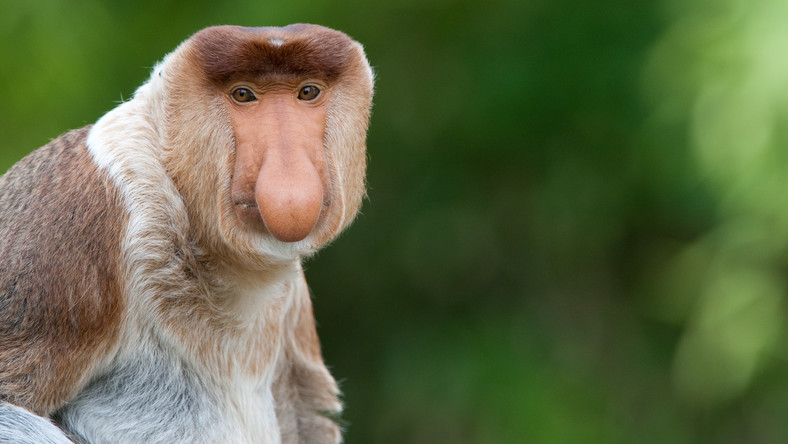
\includegraphics[scale=13]{nosacz.jpg}
\caption{NOSACZ \cite{Wiki}}
\label{nosacz}
\end{figure}
\end{frame}

\begin{frame}{Kret}
\begin{figure}[h!]
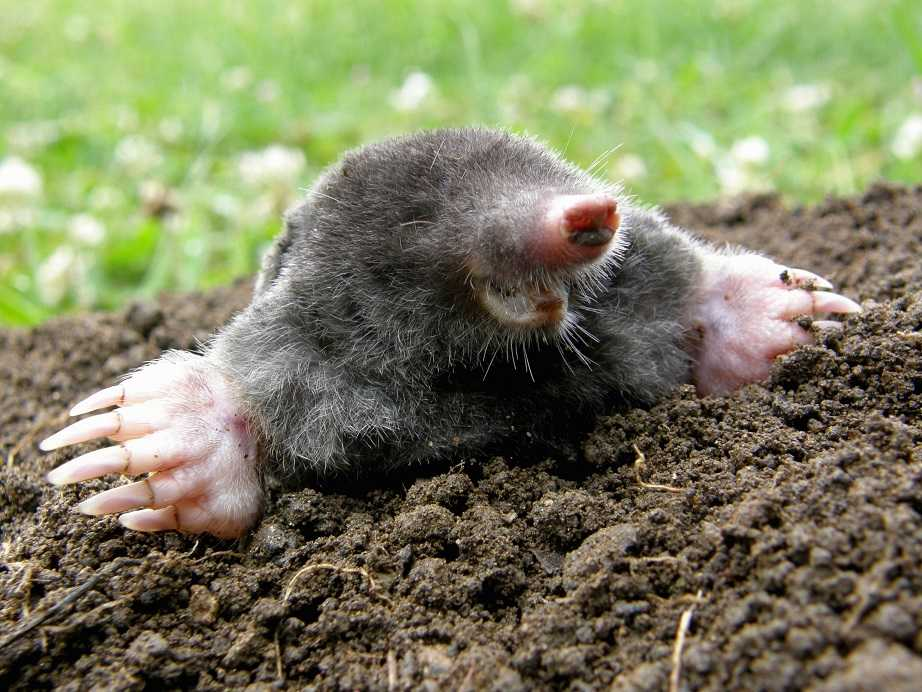
\includegraphics[scale=2]{kret.jpg}
\caption{Kret \cite{Wiki}}
\label{kret}
\end{figure}
\end{frame}

\begin{frame}{Kotek}
\begin{figure}[h!]
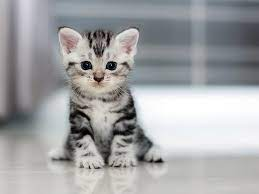
\includegraphics[scale=0.7]{kotek.jpg}
\caption{Kotek \cite{Wiki}}
\label{kotus}
\end{figure}
\end{frame}

\begin{frame}{Puszyste}
\begin{enumerate}[a)]
\item Kotek
\pause
\item Kret
\pause
\item Sloniopodobny
\end{enumerate}
\end{frame}

\begin{frame}{Konik}
\begin{figure}[h!]
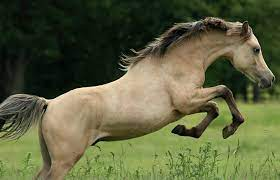
\includegraphics[scale=0.3]{konik.jpg}
\end{figure}
\end{frame}

\begin{frame}{Konik}
\begin{figure}[h!]
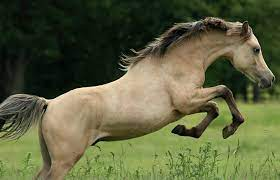
\includegraphics[scale=0.5]{konik.jpg}
\end{figure}
\end{frame}

\begin{frame}{Nosacz}
\begin{figure}[h!]
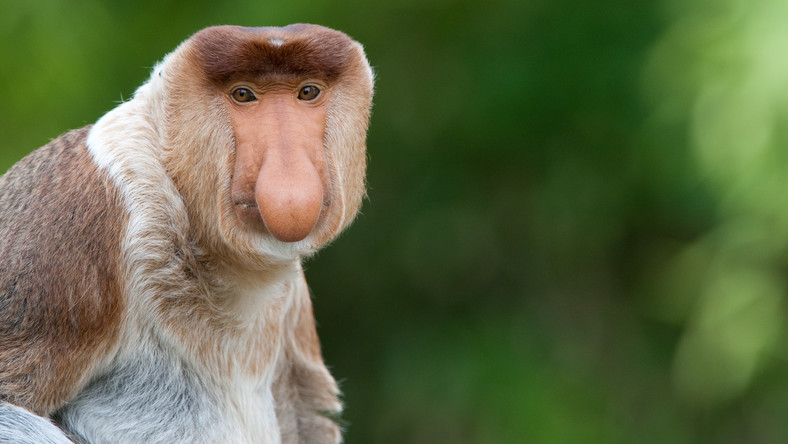
\includegraphics[scale=0.5]{nosacz.jpg}
\end{figure}
\end{frame}

\begin{frame}{Odwołania}
Plum \cite{Miotk}
\begin{enumerate}[a)]
\item Tabela \ref{t1} no tutaj cos tam 
\pause
\item Obraz \ref{nosacz} NOSACZ@@@@@!!!!
\pause
\item Obrazekk  \ref{kret} pokazuje krecika
\pause
\item Obraz \ref{kotus} kotus
\end{enumerate}
\end{frame}

\begin{frame}{Bibliografia}
\section{Bibliografia}\label{bb}
\begin{thebibliography}{2}
\bibitem{Miotk}
blabla \LaTeX \footnote[1]{nie lubie latexa}"
\bibitem{Wiki}
Zdjęcia: internet\footnote[2]{kradzione!!!}
\end{thebibliography}
\end{frame}

\end{document}